%%% File encoding: UTF-8
%%% äöüÄÖÜß  <-- keine deutschen Umlaute hier? UTF-faehigen Editor verwenden!

\documentclass[foo,german]{hgbthesis}
% Zulässige Class Options:
%   Typ der Arbeit: diplom, master (default), bachelor, praktikum
%   Hauptsprache: german (default), english
%%%----------------------------------------------------------

\RequirePackage[utf8]{inputenc}		% Bei der Verw. von lualatex oder xelatex entfernen!

\graphicspath{{images/}}    % Abbildungsverzeichnis
\logofile{}				% Name des Logo-PDFs in images/ (\logofile{}, wenn kein Logo gewünscht)
\bibliography{literatur}  	% Name der Biblatex-Literaturdatei (.bib)

%%%----------------------------------------------------------
% Angaben für die Titelei (Titelseite, Erklärung etc.)
%%%----------------------------------------------------------

%%% Einträge für ALLE Arbeiten: -----------------------------
\title{Linux on z; Was unterscheidet Linux on z zu einem Linux auf x86}
\author{Timo Furrer}
\studiengang{Mainframe Topics Blockwoche}
\studienort{Hochschule Luzern}
\abgabedatum{2017}{09}{10}	% {YYYY}{MM}{DD}

%%% Zusätzlich für eine Bachelorarbeit: ---------------------
\nummer{XXXXXXXXXX-A}   % Stud-ID, z.B. 1310238045-A
% (A = 1. Bachelorarbeit)
\semester{Sommersemester 2016}
\gegenstand{Einführung in die Tiefere Problematik 1}
\betreuer{Alois B.~Treuer, Päd.\ Phil.} % oder \betreuerin{..}

%%% Restriktive Lizenformel anstatt CC (nur für Typ master) -
%\strictlicense

%%%----------------------------------------------------------
\begin{document}
%%%----------------------------------------------------------

%%%----------------------------------------------------------
\frontmatter                    % Titelei (röm. Seitenzahlen)
%%%----------------------------------------------------------

\maketitle
\tableofcontents

%\chapter{Vorwort} 	% engl. Preface


Dies ist \textbf{Version \hgbthesisDate} der \latex-Dokumentenvorlage für 
verschiedene Abschlussarbeiten an der Fakultät für Informatik, Kommunikation
und Medien der FH Oberösterreich in Hagenberg, die mittlerweile auch 
an anderen Hochschulen im In- und Ausland gerne verwendet wird.

Das Dokument entstand ursprünglich auf Anfragen von Studierenden,
nachdem im Studienjahr 2000/01 erstmals ein offizieller
\latex-Grundkurs im Studiengang Medientechnik und -design an der
FH Hagenberg angeboten wurde. Eigentlich war die Idee, die bereits
bestehende \emph{Word}-Vorlage für Diplomarbeiten "`einfach"' in
\latex\ zu übersetzen und dazu eventuell einige spezielle
Ergänzungen einzubauen. Das erwies sich rasch als wenig
zielführend, da \latex, \va was den Umgang mit Literatur und
Grafiken anbelangt, doch eine wesentlich andere Arbeitsweise
verlangt. Das Ergebnis ist -- von Grund auf neu geschrieben und
wesentlich umfangreicher als das vorherige Dokument --
letztendlich eine Anleitung für das Schreiben mit \latex, ergänzt
mit einigen speziellen (mittlerweile entfernten) Hinweisen für \emph{Word}-Benutzer.
Technische Details zur aktuellen Version finden sich in Anhang \ref{ch:TechnischeInfos}.

Während dieses Dokument anfangs ausschließlich für die Erstellung
von Diplomarbeiten gedacht war, sind nunmehr auch  
\emph{Masterarbeiten}, \emph{Bachelor\-arbeiten} und \emph{Praktikumsberichte} 
abgedeckt, wobei die Unterschiede bewusst gering gehalten wurden.

Bei der Zusammenstellung dieser Vorlage wurde versucht, mit der
Basisfunktionalität von \latex das Auslangen zu finden und -- soweit möglich --
auf zusätzliche Pakete zu verzichten. Das ist nur zum Teil gelungen;
tat\-säch\-lich ist eine Reihe von ergänzenden "`Paketen"' notwendig, wobei jedoch
nur auf gängige Erweiterungen zurückgegriffen wurde.
Selbstverständlich gibt es darüber hinaus eine Vielzahl weiterer Pakete,
die für weitere Verbesserungen und Finessen nützlich sein können. Damit kann
sich aber jeder selbst beschäftigen, sobald das notwendige Selbstvertrauen und
genügend Zeit zum Experimentieren vorhanden sind.
Eine Vielzahl von Details und Tricks sind zwar in diesem Dokument nicht explizit
angeführt, können aber im zugehörigen Quelltext jederzeit ausgeforscht
werden.

Zahlreiche KollegInnen haben durch sorgfältiges Korrekturlesen und
konstruktive Verbesserungsvorschläge wertvolle Unterstützung
geliefert. Speziell bedanken möchte ich mich bei Heinz Dobler für
die konsequente Verbesserung meines "`Computer Slangs"', bei
Elisabeth Mitterbauer für das bewährte orthographische Auge und
bei Wolfgang Hochleitner für die Tests unter Mac~OS.

Die Verwendung dieser Vorlage ist jedermann freigestellt und an
keinerlei Erwähnung gebunden. Allerdings -- wer sie als Grundlage
seiner eigenen Arbeit verwenden möchte, sollte nicht einfach
("`ung'schaut"') darauf los werken, sondern zumindest die
wichtigsten Teile des Dokuments \emph{lesen} und nach Möglichkeit
auch beherzigen. Die Erfahrung zeigt, dass dies die Qualität der
Ergebnisse deutlich zu steigern vermag.

Der Quelltext zu diesem Dokument sowie das zugehörige
\latex-Paket sind in der jeweils aktuellen Version online
verfügbar unter
%
\begin{itemize}
\item[]\url{https://sourceforge.net/projects/hgbthesis/}.
\end{itemize}
%
Trotz großer Mühe enthält dieses Dokument zweifellos Fehler und Unzulänglichkeiten
-- Kommentare, Verbesserungsvorschläge und passende Ergänzungen
sind daher stets willkommen, am einfachsten per E-Mail direkt an mich:
\begin{itemize}
\item[]%

Dr.\ Wilhelm Burger, Department für Digitale Medien,\newline
Fachhochschule Oberösterreich, Campus Hagenberg (Österreich)\newline
\nolinkurl{wilhelm.burger@fh-hagenberg.at}
\end{itemize}

\noindent
Übrigens, hier im Vorwort (das bei Diplom- und Masterarbeiten üblich, bei Bachelorarbeiten 
aber entbehrlich ist) kann kurz auf die Entstehung des Dokuments eingegangen werden.
Hier ist auch der Platz für allfällige Danksagungen (\zB an den Betreuer, 
den Begutachter, die Familie, den Hund, \ldots), Widmungen und philosophische 
Anmerkungen. Das sollte allerdings auch nicht übertrieben werden und sich auf 
einen Umfang von maximal zwei Seiten beschränken.




 % Optional. Ggf. weglassen
%\chapter{Kurzfassung}

An dieser Stelle steht eine Zusammenfassung der Arbeit, Umfang
max.\ 1 Seite. Im Unterschied zu anderen Kapiteln ist die
Kurzfassung (und das Abstract) üblicherweise nicht in Abschnitte
und Unterabschnitte gegliedert. 
Auch Fußnoten sind hier falsch am Platz.

Kurzfassungen werden übrigens häufig -- zusammen mit Autor und Titel
der Arbeit -- %
in Literaturdatenbanken aufgenommen. Es ist daher darauf zu
achten, dass die Information in der Kurzfassung für sich 
\emph{allein} (\dah ohne weitere Teile der Arbeit) zusammenhängend und
abgeschlossen ist. Insbesondere werden an dieser Stelle (wie \ua
auch im \emph{Titel} der Arbeit und im \emph{Abstract})
normalerweise \emph{keine Literaturverweise} verwendet! Falls
unbedingt solche benötigt werden -- etwa weil die Arbeit eine
Weiterentwicklung einer bestimmten, früheren Arbeit darstellt --,
dann sind \emph{vollständige} Quellenangaben in der Kurzfassung
selbst notwendig, \zB %
[\textsc{Zobel} J.: \textit{Writing for Computer Science -- The Art of
Effective Commu\-nica\-tion}. Springer-Verlag, Singa\-pur, 1997].

Auch sollte daran gedacht werden, dass bei der Aufnahme in Datenbanken
Sonderzeichen oder etwa Aufzählungen mit "`Knödellisten"' in der
Regel verloren gehen. Dasselbe gilt natürlich auch für das 
\emph{Abstract}.


Inhaltlich sollte die Kurzfassung \emph{keine} Auflistung der
einzelnen Kapitel sein (dafür ist das Einleitungskapitel
vorgesehen), sondern dem Leser einen kompakten, inhaltlichen
Überblick über die gesamte Arbeit verschaffen. Der hier verwendete
Aufbau ist daher zwangsläufig anders als der in der Einleitung.

\chapter{Abstract}

\begin{english} %switch to English language rules
This should be a 1-page (maximum) summary of your work in English.
%und hier geht dann das Abstract weiter...
\end{english}

Im englischen Abstract sollte inhaltlich das Gleiche
stehen wie in der deutschen Kurzfassung. Versuchen Sie daher, die
Kurzfassung prä\-zise umzusetzen, ohne aber dabei Wort für Wort zu
übersetzen. Beachten Sie bei der Übersetzung, dass gewisse
Redewendungen aus dem Deutschen im Englischen kein Pendant haben
oder völlig anders formuliert werden müssen und dass die
Satzstellung im Englischen sich (bekanntlich) vom Deutschen stark
unterscheidet (mehr dazu in Abschn.\ \ref{sec:englisch}). Es
empfiehlt sich übrigens -- auch bei höchstem Vertrauen in die
persönlichen Englischkenntnisse -- eine kundige Person für das
"`proof reading"' zu engagieren.

Die richtige Übersetzung für "`Diplomarbeit"' ist übrigens
schlicht \emph{thesis}, allenfalls  "`diploma thesis"' oder "`Master's thesis"', 
auf keinen Fall aber "`diploma work"' oder gar "`dissertation"'. 
Für "`Bachelorarbeit"' ist wohl "`Bachelor thesis"' die passende Übersetzung. 

Übrigens sollte für diesen Abschnitt die \emph{Spracheinstellung} in \latex\ von Deutsch
auf Englisch umgeschaltet werden, um die richtige Form der
Silbentrennung zu erhalten, die richtigen Anführungszeichen müssen allerdings selbst gesetzt werden %
(s.\ dazu die Abschnitte \ref{sec:sprachumschaltung} %
und \ref{sec:anfuehrungszeichen}).


%%%----------------------------------------------------------
\mainmatter          % Hauptteil (ab hier arab. Seitenzahlen)
%%%----------------------------------------------------------

\chapter{Einleitung}
\label{cha:Einleitung}

\section{Was ist Linux?}

Unter dem Begriff Linux versteht man allgemein einen Ueberbegriff fuer freie Betriebssysteme, welche auf dem Linux Kernel basieren. Der Linux Kernel wurde erstmals im frühjahr 1992 unter der GNU GPL Lizenz fuer Intels x86 Architektur veroeffentlicht.

Ein konkretes Linux Betriebssystem bezeichnet man als Linux Distribution. Eine Distribution besteht aus einem Linux Kernel, GNU Tools und Libraries, zusaetzlicher Software und manchmal auch einem Window System, einem Windows Manager und einem Desktop Environment. Beispiele fuer solche Linux Distributionen sind Debian, Ubuntu, Arch Linux, openSUSE, Fedora und Linux on z.

\section{Linux Kernel Architekturen}

Der Linux Kernel ist von monolithischer aber auch modularer Natur. Dies bedeutet, dass Funktionalitaeten, welche der Kernel zwingend braucht, direkt eingebaut sind - Funktionalitaeten welche aber nur bei ganz bestimmten Hardwarekomponenten gebraucht werden, koennen ueber sogenannte Kernel Module nachgeladen werden.
Der Linux Kernel uebernimmt Aufgaben wie beispielsweise die Speicher- und Prozessverwaltung, Interprozesskommunikation, Geraeteverwaltung und Dateisystem.
Nachfolgende Grafik zeigt eine Uebersicht wichtiger Aufgaben des Linux Kernels im Zusammenspiel mit Hardware und den Userspace Anwendungen der Distribution:

\begin{figure}[h!]
\centering
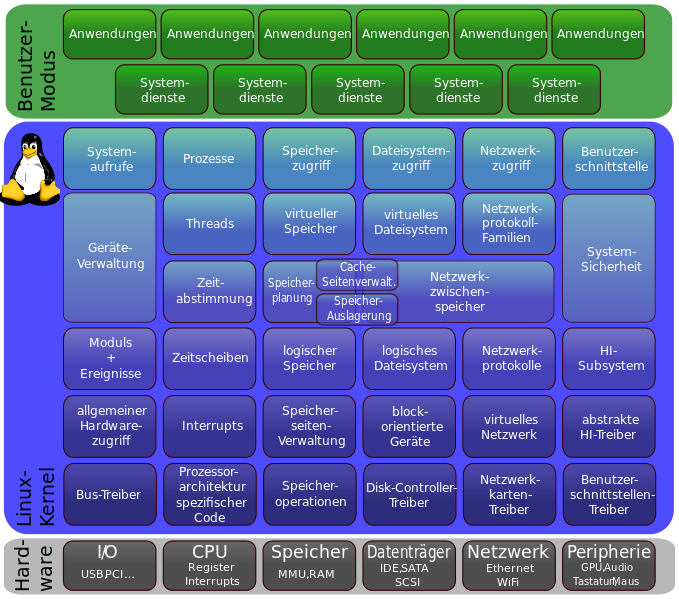
\includegraphics[width=.80\textwidth]{einleitung-kernel-struktur}
\caption{Linux Kernel Struktur\cite{KernelStruktur}.}
\label{fig:KernelStruktur}
\end{figure}

\newpage

Dieser modular-monolithischer Ansatz des Linux Kernels traegt nicht zuletzt zu seiner grossen Verbreitung auf unterschiedlichsten Architekturen und Plattformen bei.

Wikipedia fuehrt eine Liste der Computer Architekturen, welche Linux unterstuetzt.
Inzwischen sind dort ueber 100 Architekturen zu finden. Diese breite Abdeckung von Architekturen macht es moeglich, dass Linux in beinahe alle Bereiche von Betriebssystem Umgebungen Einzug gefunden hat. Diese reicht von exotischen Umgebungen, wie Navigations- und Haushaltsgeraeten, Digitalkameras, ueber Desktop- und Laptop Computern und Mobiltelefonen mit Android, bis hin zu Supercomputern und High Performance Computing Clusters mit Rocks Cluster Distribution.

So hat Linux auch seine Daseinsberechtigung auf dem Mainframe gefunden mit Linux on z, welches auf IBMs z Systems und IBMs LinuxONE laeuft.

\chapter{Fazit}
\label{cha:Schluss}

Auch wenn diese Arbeit das Aufarbeiten von nur wenigen Unterschieden zwischen Linux on x86 und Linux on z zugelassen hat, so haben die vorgängigen Kapitel gezeigt, dass es durchaus Sinn machen kann grössere Linux x86 Server Infrastrukturen auf ein Mainframe mit Linux on z zu konsolidieren.
Ich denke die Hauptgründe dafür sind:
\begin{description}
    \item[Eine Hardware]{Eine Mainframe Hardware ist in der Lage hunderte Linux on z Instanzen laufen zu lassen. Der Footprint eines IBM Mainframes erspart Platz, Strom und im Endeffekt dann vor allem auch Geld.\footnote{Siehe Abschnitt \ref{sec:Konsolidierung}}}
    \item[Workload Management]{Da die Linux on z Instanzen auf einer einzigen grossen Hardware laufen, hat ein Mainframe die Möglichkeit den Workload perfekt auf die zur Verfügung stehenden Ressourcen zu verteilen.\footnote{Siehe Abschnitt \ref{sec:WorkloadManagement}}}
    \item[Exterm performante Kommunikation]{Mit HiperSockets bietet Linux on z eine extrem performante \textit{in-memory} TCP/IP Kommunikationsschnittstelle\footnote{Siehe Abschnitt \ref{sec:HiperSockets}}}
    \item[Call Home]{Die Call Home Funktion im Linux Kernel vereinfacht das Raportieren von Kernel Panics an IBM.}
\end{description}


%%%----------------------------------------------------------
\appendix                                            % Anhang
%%%----------------------------------------------------------

%%%----------------------------------------------------------
\MakeBibliography                        % Quellenverzeichnis
%%%----------------------------------------------------------

%%% Messbox zur Druckkontrolle ------------------------------
\chapter*{Messbox zur Druckkontrolle}



\begin{center}
{\Large --- Druckgröße kontrollieren! ---}

\bigskip

\Messbox{100}{50} % Angabe der Breite/Hoehe in mm

\bigskip

{\Large --- Diese Seite nach dem Druck entfernen! ---}

\end{center}



%%%----------------------------------------------------------
\end{document}
%%%----------------------------------------------------------
